


On présente ici quelques techniques de régression plus avancées. Elles peuvent entre autres être utilisées si les postulats de la RLM ne sont pas vérifiés.


\section{Régression polynomiale}
\label{sec:regpoly}

L'idée derrière la régression linéaire est que le modèle
linéaire est une bonne approximation de la \og vraie \fg relation
entre la variable endogène et les variables exogènes
$$Y=f(x_1,x_2,\ldots,x_k)+\varepsilon.$$
Dans plusieurs cas, le modèle de régression linéaire sera
une approximation suffisamment bonne de $f(x_1,\ldots,x_k)$. Par
contre dans certaines situations, il arrive que l'approximation
linéaire ne soit pas assez proche de $f(x_1,\ldots,x_k)$ pour
donner un modèle approprié. Dans ces cas, nous pouvons
utiliser le principe disant que la plupart des fonctions peuvent
\^etre approchées aussi bien que l'on veut par une expansion
polynomiale. Plus il y a de la \og courbure \fg dans
$f(x_1,\ldots,x_k)$, plus le polyn\^ome utilisé pour
approcher $f(x_1,\ldots,x_k)$ doit \^etre de degré élevé
pour que l'approximation soit suffisamment précise.

En régression, ceci se traduit par le résultat suivant:
\begin{eqnarray*}
Y_i&=&f(x_{1i},\ldots,x_{ki})+\varepsilon_i\\
&\approx&\beta_0+\beta_1x_{1i}+\cdots+\beta_kx_{ki}\\
&\ &\ \ \ +\beta_{11}x_{1i}^2+\cdots+\beta_{kk}x_{ki}^2+
\beta_{12}x_{1i}x_{2i}+\cdots+\beta_{k-1,k}x_{k-1,i}x_{ki}\\
&\ & \ \ \ +\beta_{111}x_{1i}^3+\cdots+ \beta_{kk\cdots
k}x_{ki}^d+\cdots+\varepsilon_i.
\end{eqnarray*}
En général, il est rarement nécessaire de dépasser un modèle du second degré:
\begin{eqnarray*}
Y_i&=&\beta_0+\beta_1x_{1i}+\cdots+\beta_kx_{ki}\\
&\ &\ \ \ +\beta_{11}x_{1i}^2+\cdots+\beta_{kk}x_{ki}^2+
\beta_{12}x_{1i}x_{2i}+\cdots+\beta_{k-1,k}x_{k-1,i}x_{ki}.
\end{eqnarray*}

Il est possible que l'on rencontre des problèmes numériques ou
de multicolinéarité quand on utilise des modèles polynomiaux. Si l'objectif est de trouver un modèle faisant de bonnes prédictions, ce n'est pas vraiment un problème. Si on veut vraiment interpréter les valeurs des coefficients de chaque terme, alors on peut travailler avec les variables exogènes standardisées, c'est-à-dire de
remplacer $x_{ji}$ par
$$x_{ji}^*=\frac{(x_{ji}-\bar{x}_j)}{s_j}$$

$ \mbox{ o\`u } \bar{x_j}=\sum_ix_{ji}/n \mbox{ et } s_j^2=\sum_i(x_{ji}-\bar{x}_j)^2/(n-1).$

\subsubsection*{Sélection de modèle}

Comme c'était le cas avec les interactions, si un terme de
degré $d$ est inclus dans le modèle, alors en général on
inclut les termes de degré inférieur \`a $d$.% composés des termes présents dans le terme de degré $d$ en question.


%\noindent\textbf{Note:} Il est préférable d'utiliser une transformation de $Y$ et/ou de certains des $x$ si cette transformation donne d'aussi bons résultats qu'un modèle polynomial avec moins de paramètres. Par exemple, $$\ln Y_i=\beta_0+\beta_1x_{1i}+\varepsilon_i$$ ou $$Y_i=\beta_0+\beta_1e^{x_{1i}}+\varepsilon_i$$ peut \^etre préférable \`a $$Y_i=\beta_0+\beta_1x_{1i}+\beta_2x_{1i}^2+\beta_3x_{3i}^3+\varepsilon_i.$$ Un examen des résidus et de la valeur des critères de sélection de modèle aident souvent \`a déterminer quel modèle est le plus approprié pour vos données.


\subsubsection*{Test de comparaison de modèle pour justifier un degré supérieur}

% Tout comme c'était le cas avec les termes d'interaction, des termes de degré supérieur peuvent \^etre ajoutés \`a un modèle afin d'en vérifier l'ajustement.

\begin{exemple}
Soit le modèle
$Y=\beta_0+\beta_1x_{1}+\beta_2x_{2}+\varepsilon.$

Ce modèle est-il aussi valide que celui contenant des termes de degré 2?
$$Y=\beta_0+\beta_1x_{1}+\beta_2x_{2}+\beta_{11}x_{1}^2
+\beta_{22}x_{2}^2+ \beta_{12}x_{1}x_{2}+\varepsilon.$$

Nous pouvons utiliser un test $F$ de comparaison de modèles pour les hypothèses\\
$H_0:\ \beta_{11}=\beta_{22}=\beta_{12}=0$ contre \\
$H_1:$ au moins un de ces $\beta$ diffère de 0. \\

Si nous ne rejetons pas $H_0$, les données ne montrent pas d'amélioration significative par ces termes de second degré; les autres diagnostics restent nécessaires. Si nous rejetons $H_0$, alors le modèle de premier degré n'est pas adéquat.\\

On aurait pu vérifier l'ajout d'un seul terme à la fois, car il est fort possible qu'une relation quadratique soit souhaitable en $x_1$ mais pas en $x_2$.
\end{exemple}


\newpage

\section{Régression non linéaire}


Si l'espérance de $Y$ (ou de $g(Y)$) n'est pas une fonction linéaire des paramètres inconnus, mais qu'on a une idée de la vraie relation entre $Y$ et les variables indépendantes, on peut néanmoins estimer les paramètres de cette relation non linéaire avec la méthode des moindres carrés. Il n'y a pas de solution analytique dans ce cas, mais des  méthodes numériques peuvent minimiser la somme des carrés des erreurs.

\begin{exemple}
Dans une expérience sur des rats, on trempe  des portions du ventricule auriculaire gauche dans une solution de chlorure de calcium, puis on stimule électriquement le tissu et on mesure la longueur du rétrécissement de la bandelette de tissu.
On s'intéresse à la relation entre
\begin{itemize}
\item[] x :  la concentration de chlorure de calcium (en mM)
\item[] Y : le changement de longueur de la bandelette en réaction au choc (en mm)
\end{itemize}
La figure \ref{fig:rat1} illustre les données. Il est clair qu'un modèle linéaire n'est pas approprié.

Il se trouve toutefois qu'on a déjà une idée du modèle approprié pour les données:
$$ Y_i =  \alpha + \beta e^{-x_i / \theta} + \varepsilon_i $$
La régression non linéaire permet d'estimer les coefficients par la méthode des moindres carrés. On trouve $\hat\theta = 0,6082$, $\hat\alpha = 28,9633$ et $\hat\beta = -34,2274$. La fonction de régression correspondante est également illustrée à la figure \ref{fig:rat1}.

\begin{figure}[H]
\centering
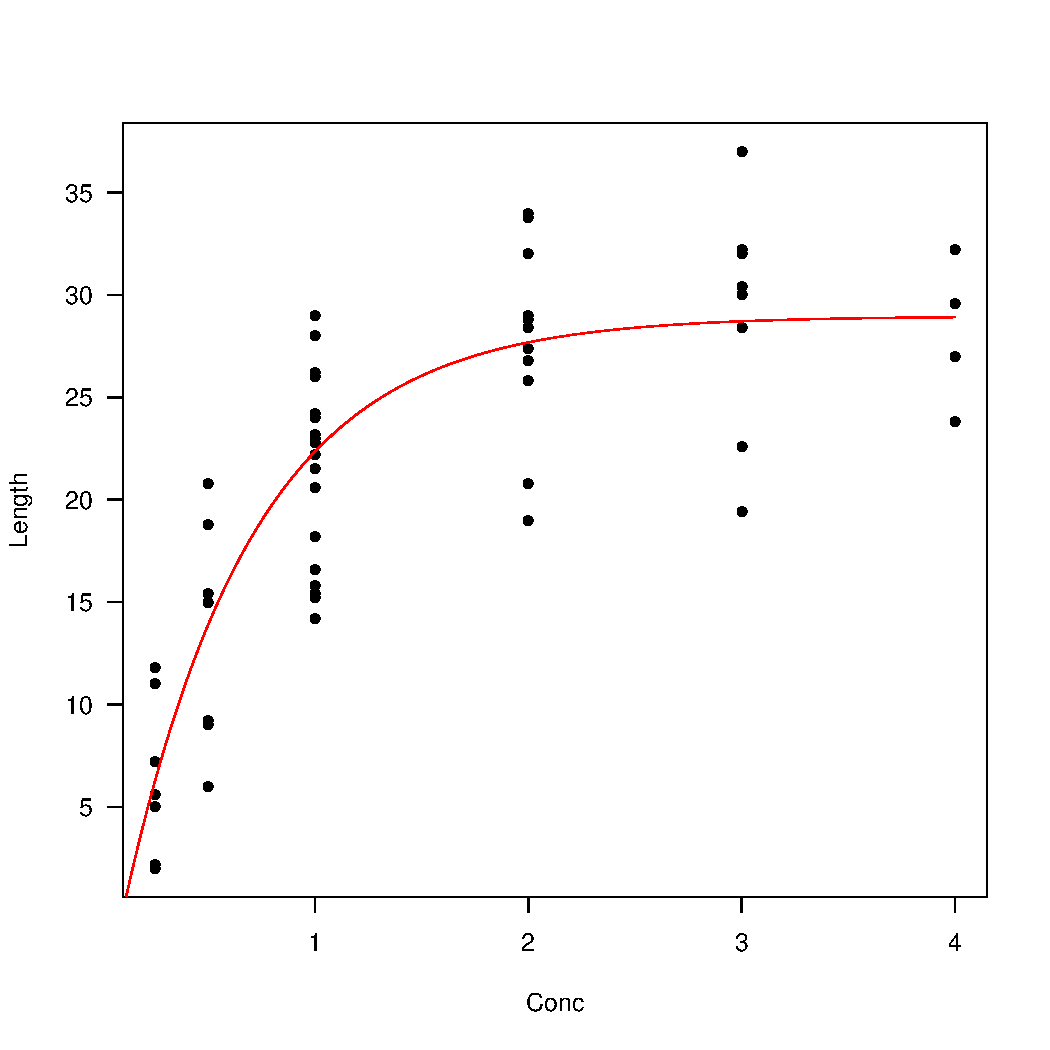
\includegraphics[scale=0.5]{Chap11-TechniquesAvancees/Figures/Nonlinear2}
\caption{Données d'une expérience sur des rats de laboratoire avec la fonction de régression estimée}
\label{fig:rat1}
\end{figure}
\end{exemple}


\newpage
\section{Régression pondérée}


La méthode des moindres carrés pondérés consiste \`a attribuer un poids différent  à chaque observation, et donc à trouver $\hat{\bobeta}$ tel que
$$\sum_{i=1}^nw_i(Y_i-\hat{Y}_i)^2$$
est minimale, o\`u $w_i$ est le poids associé à l'observation $i$.

Une application fréquente de la régression pondérée est lorsque l'hypothèse d'homo\-scédasticité n'est pas respectée, c'est-à-dire si le modèle est plutôt caractérisé par \\$\boeps\sim \mathcal{N}_n(\boz,\mbox{diag}(\sigma_1^2,\ldots,\sigma_n^2))$, o\`u les $\sigma_i^2$ ne sont pas nécessairement égaux.


Le choix des poids $w_i$ n'est pas toujours facile à faire. Si chaque observation est en réalité la moyenne de $n_i$ valeurs, on peut utiliser un poids égal $w_i=n_i$. Si la variance des erreurs est liée à une variable explicative, on peut faire un graphe des paires $(x_i,\, t_i)$, et voir
comment la variance des résidus studentisés évolue en
fonction de $x_i$. Si le graphe est en forme d'entonnoir ouvert
vers la droite, alors on pourra prendre $w_i=1/x_i$,
$w_i=1/\sqrt{x_i}$, $w_i=1/x_i^{2}$, etc. Si l'entonnoir ouvre vers
la gauche, alors on peut prendre $w_i=x_i$, $w_i=\sqrt{x_i}$,
$w_i=x_i^{2}$, etc. Il est toutefois recommandé d'essayer d'abord de régler le problème à l'aide d'une transformation de variable.

En régression linéaire multiple, il y a plusieurs variables explicatives, il faut donc trouver une stratégie plus globale en cas d'hétéroscédasticité. 
L'idéal serait d'identifier des poids de la forme $w_i\propto1/\sigma^2_i \;$, où $\sigma_i^2$ est la variance de l'erreur pour l'observation $i$. On peut démontrer que dans ce cas,
$$\hat{\bobeta}=(\boX'\boV^{-1}\boX)^{-1}\boX'\boV^{-1}\boY,$$
o\`u $\boV=\mbox{diag}(\sigma_1^2,\ldots,\sigma_n^2)$. La variance de
$\hat{\bobeta}$ est alors
\begin{eqnarray*}
\var(\hat{\bobeta})&=&(\boX'\boV^{-1}\boX)^{-1}\boX'\boV^{-1}\;\boV\;\boV^{-1}\boX(\boX'\boV^{-1}\boX)^{-1}\\
&=&(\boX'\boV^{-1}\boX)^{-1}.
\end{eqnarray*}
Si $\boV$ est connue, la statistique obtenue en divisant
$\hat\beta_j-c$ par son écart-type connu suit une loi normale standard sous
$H_0$. Si $\boV=\sigma^2\bo{W}^{-1}$ avec $\bo{W}$ connue et $\sigma^2$
inconnue, on estime $\sigma^2$ par
\[
 s_W^2=\frac{\sum_i w_i(Y_i-\hat Y_i)^2}{n-p'}.
\]
Sous normalité, la statistique
$(\hat\beta_j-c)/\{s_W\sqrt{(\boX'\bo{W}\boX)^{-1}_{jj}}\}$ suit alors
une loi de Student à $n-p'$ degrés de liberté. Si les poids sont estimés à
partir des mêmes données, ces résultats sont généralement approchés.

Or, établir des estimations des $\sigma_i$ n'est pas si évident.  Voici quelques pistes de solutions (il faut d'abord ajuster une régression du modèle complet et s'assurer que la linéarité est respectée):

\begin{itemize}
\item Si le graphique des $\hat\varepsilon_i$ en fonction des $\hat Y_i$ est en entonnoir, on ajuste une régression des $|\hat\varepsilon_i|$ sur les $\hat Y_i$. Les valeurs prédites de ce nouvel ajustement sont une estimation de $\sigma_i$. (Et les poids seront $w_i=1/\hat\sigma_i^2$).

\item Si le graphique des $\hat\varepsilon_i^2$ en fonction des $\hat Y_i$ montre une tendance à la hausse, on ajuste une régression des $\hat\varepsilon_i^2$ sur les $\hat Y_i$. Les valeurs prédites de ce nouvel ajustement sont une estimation de $\sigma_i^2$. (Et les poids seront $w_i=1/\hat\sigma_i^2$).
% Source: https://onlinecourses.science.psu.edu/stat501/node/352
\end{itemize}
%Parfois on utilise $\boV=\boV^*\sigma^2$ et on estime $\sigma^2$ par $$s^2={\sum_{i=1}^nw_i(Y_i-\hat{Y}_i)^2\over n-p'}.$$

% Une table d'analyse de variance peut aussi \^etre construite en utilisant la décomposition
% $$ {\underbrace{\boY'\boV^{-1}\boY}\atop SC_{tot:W}}={\underbrace{\hat{\bobeta}\boX'\boV^{-1}\boY} \atop SC_{reg:W}}+{\underbrace{(\boY-\boX\hat{\bobeta})'\boV^{-1}(\boY-\boX\hat{\bobeta})} \atop SC_{res:W}}.$$ 

Quelques remarques sur la régression pondérée:
\begin{itemize}
\item En général, les estimations des $\hat\beta_j$ ne seront pas dramatiquement changées par la régression pondérée.
\item Les degrés de liberté ne sont pas affectés par l'insertion de poids. %calculés de la m\^eme fa\c{c}on qu'en régression linéaire ordinaire.
\item Les intervalles de confiance et les tests d'hypothèses sont affectés par les poids.
% Source: https://onlinecourses.science.psu.edu/stat501/node/352
\end{itemize}

\newpage

\section{Modélisation de la dépendance}

Lorsque l'hypothèse d'indépendance des observations n'est pas vérifiée, on peut modéliser directement la dépendance en ajoutant des paramètres à la matrice de covariance des erreurs. Alors que la régression pondérée permet des valeurs différentes sur la diagonale de la matrice de covariance des erreurs, on modélise la dépendance en remplaçant les zéros hors diagonale par des paramètres à estimer. Selon la dépendance que l'on souhaite modéliser, on paramétrisera la matrice de covariance différemment.


Une forme particulière de dépendance est l'autocorrélation, qui arrive lorsque le résidu d'une observation est relié à celui de l'observation précédente, par exemple dans une série temporelle. Un modèle dit autorégressif peut alors être utilisé pour ajuster un modèle de régression.

Mathématiquement, on écrit
\begin{equation}\label{ar1}
\varepsilon_i=\rho\varepsilon_{i-1}+u_i, \end{equation} o\`u
les innovations $u_i$ sont i.i.d. $\mathcal{N}(0,\sigma_u^2)$. Le paramètre
$\rho$ dans (\ref{ar1}) est nommé paramètre
d'au\-to\-cor\-ré\-la\-tion, et sa valeur doit \^etre dans
l'intervalle (-1,1).

En supposant le processus stationnaire, avec $\varepsilon_1\sim\N(0,\sigma_u^2/(1-\rho^2))$ indépendant des innovations futures, à partir de (\ref{ar1}), nous pouvons
calculer directement que
\begin{eqnarray*}
\varepsilon_i&=&\sum_{j=0}^\infty\rho^ju_{i-j}\\
\esp[\varepsilon_i]&=&\sum_{j=0}^\infty\rho^j\esp[u_{i-j}]=0\\
\var[\varepsilon_i]&=&\sigma_u^2\sum_{j=0}^\infty\rho^{2j}={\sigma_u^2\over1-\rho^2}\\
\cov(\varepsilon_i,\varepsilon_{i+j})&=&\rho^{|j|}{\sigma_u^2\over1-\rho^2}.
\end{eqnarray*}
Comme on peut le voir, une autocorrélation positive entre
$\varepsilon_i$ et $\varepsilon_{i+1}$ est obtenue lorsque $\rho>0$,
tandis que $\rho<0$ donne une autocorrélation négative. Il n'y a
pas d'autocorrélation lorsque $\rho=0$.



%\section{Régression non-paramétrique}

\section{Autres}

Il existe plusieurs autres modèles de régression plus complexes, notamment la régression linéaire mixte, la régression linéaire locale, la régression non-paramétrique, les arbres de régression, etc. 